%==============================================================================
%  ESGenuine — ICMLDE 5.0 submission
%  Elsevier Procedia Computer Science format
%
%  BEFORE YOU COMPILE
%  ------------------
%  1. Download the official Procedia CS template from CMT and copy `ecrc.sty`
%     (plus elsarticle.cls if your TeX distribution lacks it) NEXT TO THIS FILE.
%     Do not rely on this preamble matching the current template byte-for-byte —
%     always start from the template the conference ships and paste the body in.
%  2. This is the DOUBLE-BLIND version: authors/affiliations are anonymised and
%     there is no repository URL. Keep it that way for submission.
%  3. Every \FILL{...} is a hole that must be closed before submitting.
%  4. Compile:  pdflatex main && bibtex main && pdflatex main && pdflatex main
%
%  Target 8 pages. Limit is 3–10; beyond 10 costs INR 1,100/page.
%==============================================================================

\documentclass[3p,times]{elsarticle}

% ecrc.sty ships with the Procedia template. The \IfFileExists guard lets the
% file compile as a plain elsarticle draft while you wait for the template, so
% you are never blocked on it.
\IfFileExists{ecrc.sty}{%
  \usepackage{ecrc}
  \volume{00}
  \firstpage{1}
  \journalname{Procedia Computer Science}
  \runauth{}
  \jid{procs}
  \jnltitlelogo{Procedia Computer Science}
  \CopyrightLine{2026}{Published by Elsevier B.V.}
}{%
  \typeout{^^JWARNING: ecrc.sty not found — compiling as plain elsarticle.^^J}
}

\usepackage{graphicx}
\usepackage{booktabs}
\usepackage{amsmath}
\usepackage{multirow}
\usepackage{xcolor}
\usepackage[hidelinks]{hyperref}

% Visible placeholder — impossible to miss in the PDF.
\newcommand{\FILL}[1]{\textcolor{red}{\textbf{[FILL: #1]}}}
% Not-significant marker used in the results tables.
\newcommand{\ns}{\textsuperscript{\itshape n.s.}}
% "no errors observed" marker
\newcommand{\noerr}{\textsuperscript{$\dagger$}}

\begin{document}

\begin{frontmatter}

\dochead{5th International Conference on Machine Learning and Data Engineering}

\title{Cheap Deterministic Repair Beats Model Scale for ESG Claim Extraction:\\
An Ablation Across Disclosure Regimes}

%------------------------------------------------------------------ DOUBLE BLIND
% Restore for the camera-ready ONLY.
\author{}
\address{}
%--------------------------------------------------------------------------------

\begin{abstract}
Corporate ESG reports are audited today at the level of the document, not the
claim, which leaves individual quantitative assertions unverifiable at scale.
Large language models extract such claims readily but produce free-text
categories, misaligned fiscal-year values and page furniture that poison every
downstream use. We present a claim-extraction pipeline in which a large language
model is followed by a purely deterministic post-correction layer: taxonomy
normalisation, fiscal-year column repair, source-value verification, rule-based
aspect and type correction, and a page-furniture filter. We ablate the five
components on two sustainability reports drawn from different disclosure
regimes---an Indian statutory BRSR filing and a narrative investor-relations
report---and report 95\,\% confidence intervals from a paired bootstrap.

The deterministic layer is worth $+24.6$ and $+7.0$ points of a precision
composite over a baseline that already includes vocabulary mapping, at
$0.58$\,ms per claim and zero inference cost. Two findings are of practical
consequence. First, only two of the five components contribute measurably; the
other three are indistinguishable from zero on both documents. Second, and
centrally, \emph{which} component dominates is determined by the disclosure
regime: the rule-based gate carries the statutory filing ($+20.5$
[$+16.3$,$+25.2$]) while taxonomy normalisation carries the narrative report
($+10.6$ [$+7.8$,$+13.5$]), and the two intervals do not overlap. We further show
that precision-oriented repair is a trade rather than a free gain: over the same
stages, mechanically measured table-fact recall falls from $59.5\,\%$ to
$54.0\,\%$. All reported figures recompute offline from committed fixtures.
\end{abstract}

\begin{keyword}
ESG disclosure \sep claim extraction \sep information extraction \sep
document AI \sep greenwashing \sep large language models
\end{keyword}

\end{frontmatter}

%==============================================================================
\section{Introduction}
%==============================================================================

Corporate environmental, social and governance (ESG) reporting has grown into a
substantial disclosure regime, yet the instruments used to assess it operate at
the level of the whole document. Commercial ESG ratings compress hundreds of
pages into a single grade, and those grades disagree sharply with one another:
across six major providers, pairwise correlations average around
$0.54$~\cite{berg2022aggregate}. When raters disagree this much, a rating cannot
serve as ground truth about a firm's disclosures, and the disagreement itself
motivates a different unit of analysis---the individual claim.

A claim-level view asks a narrower and more tractable question. Rather than
``how sustainable is this company?'', it asks: what exactly did this report
assert, on which page, with what number and unit, and is that assertion
internally consistent? Answering it at scale requires turning a PDF into
structured, individually addressable claims.

Large language models make the extraction step easy and the \emph{normalisation}
step hard. An LLM asked to extract ESG claims returns fluent, largely correct
free text: it will report ``GHG emissions'' where a downstream system needs
\texttt{emissions.scope1.co2e}, will read the FY24 cell when the row label says
FY23, and will confidently emit page footers and statutory form questions as
though they were disclosures. These are not fluency failures that a larger model
obviously fixes; they are failures of alignment to a controlled vocabulary and of
document-structural awareness.

This paper examines the layer that sits between raw LLM output and a usable claim
store. Our pipeline applies five deterministic post-corrections, none of which
invokes a model or a network. The contribution is not the pipeline itself but the
measurement of that layer:

\begin{enumerate}
\item A stage-wise ablation of the deterministic layer on two documents from
      different disclosure regimes, with 95\,\% confidence intervals from a
      \emph{paired} bootstrap (Section~\ref{sec:ablation}).
\item The finding that the dominant component is determined by disclosure regime,
      with non-overlapping intervals---so a pipeline tuned on one regime
      under-serves the other.
\item A recall measure for tabular disclosures that requires no human
      annotation, derived mechanically from parsed table structure, and the
      resulting observation that precision-oriented repair \emph{costs} recall
      (Section~\ref{sec:recall}).
\item A reproducibility construction in which raw LLM outputs and parsed page
      markdown are committed as frozen fixtures, so every number reported here
      recomputes offline, deterministically, at zero API cost.
\end{enumerate}

We are explicit throughout about what the evaluation does not support. Both
annotated sets are development sets rather than held-out test sets, the composite
metric contains no recall term, and the annotation is single-annotator.
Section~\ref{sec:limitations} treats these in detail rather than deferring them
to a footnote.

%==============================================================================
\section{Related work}
%==============================================================================

\paragraph{Domain language models.} ClimateBERT~\cite{webersinke2021climatebert}
further pretrains a transformer on over two million climate-related paragraphs
and reports error reductions of $3.57\,\%$ to $35.71\,\%$ across downstream
climate NLP tasks, establishing that general-purpose models under-represent this
domain's language. Our work is complementary and deliberately model-agnostic: we
hold the extractor fixed and ask what a deterministic layer adds on top, so the
contribution transfers to whichever extractor is current.

\paragraph{Claim detection and verification.} Environmental claim
detection~\cite{stammbach2023environmental} introduces the task of identifying
environmental claims in firm communications, with an expert-annotated dataset.
Climate-FEVER~\cite{diggelmann2020climatefever} adapts fact-verification to
real-world climate claims. Both address \emph{whether a span is a claim} or
\emph{whether a claim is true}; we address the intermediate and comparatively
neglected problem of turning a detected claim into a normalised, comparable
record---the correct taxonomy node, value, unit family and claim type---which is
a precondition for either task operating over quantitative disclosures at scale.

\paragraph{LLM tools over sustainability reports.}
ChatReport~\cite{ni2023chatreport} automates sustainability-report analysis
against TCFD recommendations using LLMs with traceable answers, and releases
analyses of 1{,}015 reports. It targets question answering over reports, where
the output is prose grounded in retrieved passages. We target structured
extraction, where the output must be a normalised record that supports numeric
comparison across reports and years; the failure modes and therefore the required
corrections differ.

\paragraph{Document structure.} Layout-aware conversion is a prerequisite for
tabular disclosures. Docling~\cite{auer2024docling} converts PDFs to structured
Markdown using specialised layout and table-structure models. We use it both as a
parser and, less conventionally, as an \emph{evaluation instrument}: because it
emits tables with row labels and column headers intact, the numeric facts on a
page are mechanically enumerable, which yields a recall denominator that requires
no annotation (Section~\ref{sec:recall}).

\paragraph{Positioning.} To our knowledge the specific question here---how much of
LLM extraction error on ESG disclosures is recoverable by deterministic
post-correction, and whether the answer depends on disclosure format---has not
been measured. \FILL{if a reviewer of an adjacent venue would expect a specific
prior system, add it; a missing obvious citation is a common reject reason}

%==============================================================================
\section{System}
%==============================================================================

The pipeline is a conventional extractor followed by the layer under study.

\paragraph{Parsing.} Reports are converted with a layout-aware
parser~\cite{auer2024docling}. Text is repaired for mojibake, segmented into
sentences with provenance (page, block, bounding box), and grouped into sections;
tables are emitted separately as GitHub-flavoured Markdown with row labels and
column headers preserved.

\paragraph{Extraction.} Section windows and table pages are passed to a
large language model (\texttt{llama-3.3-70b-instruct}, temperature $0.1$) which
returns candidate claims as JSON: a free-text aspect, an action, a metric value
and unit, optional time and location, and the source sentence. Claims are
validated against a schema; malformed records are discarded.

\paragraph{Deterministic post-correction.} The layer under study applies five
cumulative corrections, none of which calls a model or the network:

\begin{description}\itemsep2pt
\item[S1 Ontology.] The free-text aspect is normalised to a node in an ESG
  taxonomy, and canonical metric family and metric key are derived. Without
  this, LLM output cannot be compared across documents at all.
\item[S2 Fiscal-year repair.] Where a table row label names a fiscal year that
  differs from the column the value was read from, the value is re-read from the
  correct column using the parsed table markdown.
\item[S3 Source-value verification.] Table claims whose value does not occur in
  the source table are flagged as potential fabrications.
\item[S4 Gate corrections.] Rule-based repairs and suspicion flags: scope
  inferred from row text, diversity/biodiversity confusion, waste/water
  confusion, implausible unit--aspect pairs, and commitment phrasing promoting a
  performance claim to a target.
\item[S5 Furniture filter.] Statutory form questions, bare row labels with
  invented numbers, and page furniture are dropped.
\end{description}

We denote by \textbf{S0} the condition in which no deterministic layer is applied
and each claim retains the model's own free-text aspect. S5 is the shipped
configuration.

%==============================================================================
\section{Evaluation setup}
%==============================================================================

\subsection{Corpus}

\FILL{confirm against the live corpus before submitting} The corpus comprises
\FILL{N} extracted claims from \FILL{N} sustainability reports across \FILL{N}
companies, spanning statutory BRSR filings, narrative investor-relations reports
and tabular ESG datasheets.

Evaluation uses two documents in depth, chosen because they sit at opposite ends
of the disclosure-format spectrum: a \textbf{statutory BRSR filing} (form-heavy,
373 raw claims) and a \textbf{narrative investor-relations report} (247 raw
claims).

\subsection{Annotated sets}

Two hand-labelled sets of 50 claims each. For every record we label whether it is
a genuine ESG claim, the correct taxonomy node, value, unit family and claim
type, read from the claim's source sentence; table values are additionally
verified against the parsed table cell. Multi-value rows from which no single
value can be pinned are marked ambiguous and excluded from strict value accuracy.

\textbf{Both sets are development sets, not held-out test sets.} The taxonomy and
repair rules were tuned against both. We report them as such throughout and
discuss the consequence in Section~\ref{sec:limitations}. All 100 labels are
single-annotator.

\subsection{Metrics}

We report six per-field rates and their unweighted mean, which we name
\texttt{precision\_composite} to make its nature explicit: \emph{candidate
precision} (of emitted claims, the share that are genuine rather than furniture
or fabrication), \emph{aspect node} and \emph{aspect pillar} accuracy,
\emph{value} accuracy within $5\,\%$ relative tolerance, \emph{unit family}
canonicalisation and \emph{claim type}.

All six are precision-family and the composite contains \textbf{no recall term}.
This is structural rather than an oversight: the annotated sets are sampled from
claims the extractor emitted, so a claim the system missed cannot appear in them.
We therefore measure recall separately and report the pair.

\subsection{Recall without human annotation}
\label{sec:recall-method}

Because the parser emits each page as Markdown with row labels and column headers
intact, the numeric facts on a page are mechanically enumerable as
$(\textit{row\_label}, \textit{column\_header}, \textit{value})$ triples. This
gives a recall denominator that is independent of the system under test and costs
no annotation.

We report \emph{distinct-fact recall}: repeated (row label, value) pairs across
column groups collapse to one fact, and governance-form cells---which carry
numbers but assert no ESG quantity---are excluded. The measure is conservative by
construction, since the denominator still contains non-claim cells such as office
counts, so true recall is at least what we report. It covers the tabular surface
only; narrative-claim recall requires human annotation and remains open.

\subsection{Statistics}

Confidence intervals are percentile bootstrap over annotated claims (2{,}000
resamples, the claim as sampling unit). Ablation deltas use a \emph{paired}
bootstrap: both stages are scored on the same resampled claims, which respects
the design---every stage is evaluated on identical data---and avoids the
needlessly wide intervals an unpaired comparison would give.

\subsection{Reproducibility}

Embedding and inference weights are pinned to specific commit revisions and all
random number generators seeded. The extraction LLM is a hosted endpoint at
non-zero temperature and is therefore not reproducible in the strict sense; we
mitigate this by committing the raw LLM outputs and parsed page markdown as
frozen fixtures, so every ablation, recall and baseline figure recomputes
exactly, offline, in seconds, at zero API cost.

%==============================================================================
\section{Results}
%==============================================================================

\subsection{Extraction quality}

Table~\ref{tab:metrics} reports per-field rates for the shipped configuration.

\begin{table*}[t]
\centering
\caption{Per-field accuracy for the shipped configuration, with 95\,\% bootstrap
confidence intervals. \noerr{}No errors were observed in the annotated sample; a
percentile bootstrap on all-correct data returns a degenerate interval, so we
report the observation rather than a point estimate of $100\,\%$. A one-sided
rule-of-three bound gives $\approx\!92\,\%$ at $n=37$.}
\label{tab:metrics}
\begin{tabular}{lccc@{\hskip 18pt}ccc}
\toprule
& \multicolumn{3}{c}{\textbf{Statutory BRSR filing}} & \multicolumn{3}{c}{\textbf{Narrative IR report}}\\
\cmidrule(r{12pt}){2-4}\cmidrule{5-7}
Metric & Point & 95\,\% CI & $n$ & Point & 95\,\% CI & $n$\\
\midrule
Candidate precision & 86.0\,\% & [75.0, 95.5] & 43 & 98.0\,\% & [94.0, 100.0] & 50\\
Aspect node         & 94.6\,\% & [85.7, 100.0] & 37 & 79.6\,\% & [68.0, 90.0] & 49\\
Aspect pillar       & no err.\noerr & --- & 37 & 89.8\,\% & [80.9, 98.0] & 49\\
Value ($\pm5\,\%$)  & no err.\noerr & --- & 12 & 97.6\,\% & [92.5, 100.0] & 42\\
Unit family         & no err.\noerr & --- & 30 & 77.3\,\% & [64.4, 89.1] & 44\\
Claim type          & no err.\noerr & --- & 37 & 95.9\,\% & [89.8, 100.0] & 49\\
\midrule
\textbf{Precision composite} & \textbf{96.1} & \textbf{[93.5, 98.5]} & 50 & \textbf{89.7} & \textbf{[85.3, 94.0]} & 50\\
\bottomrule
\end{tabular}
\end{table*}

The two composites' intervals overlap, so \textbf{we do not claim a difference in
extraction quality between the two documents}. Figure~\ref{fig:metrics} shows
where the difficulty actually differs: the narrative report is harder for
aspect-node assignment and unit canonicalisation, the statutory filing for
candidate precision, because statutory forms generate furniture that reads
superficially like disclosure.

\begin{figure*}[t]
\centering
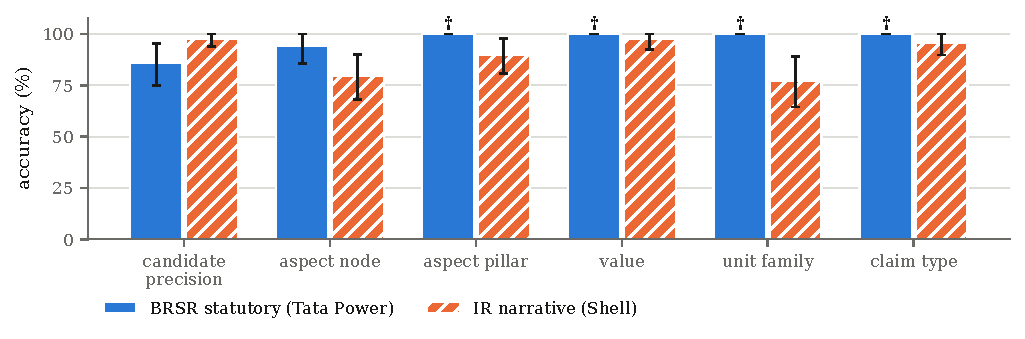
\includegraphics[width=\textwidth]{figures/fig3_per_metric_by_regime.pdf}
\caption{Per-field accuracy for the shipped configuration with 95\,\% bootstrap
confidence intervals. $\dagger$ marks rates with no observed errors, where the
percentile bootstrap returns a degenerate interval.}
\label{fig:metrics}
\end{figure*}

\subsection{Ablation: which component earns the gain}
\label{sec:ablation}

\begin{table}[t]
\centering
\caption{Cumulative precision composite by stage.}
\label{tab:stages}
\begin{tabular}{lcc}
\toprule
Stage & BRSR & IR\\
\midrule
S0 raw LLM            & 67.7 & 72.1\\
S1 $+$ ontology       & 71.5 & 82.7\\
S2 $+$ FY repair      & 73.2 & 82.7\\
S3 $+$ value-in-table & 73.2 & 82.7\\
S4 $+$ gate fixes     & 93.7 & 89.7\\
\textbf{S5 $+$ furniture drop} & \textbf{96.1} & \textbf{89.7}\\
\bottomrule
\end{tabular}
\end{table}

\begin{table}[t]
\centering
\caption{Marginal contribution per stage, paired bootstrap, 95\,\% CI.
\ns{}~indicates an interval containing zero.}
\label{tab:deltas}
\begin{tabular}{lcc}
\toprule
$\Delta$ & BRSR & IR\\
\midrule
S0$\to$S1 ontology       & $+3.8$ [1.5, 6.5]  & $\mathbf{+10.6}$ [7.8, 13.5]\\
S1$\to$S2 FY repair      & $+1.7$\ns          & $+0.0$\ns\\
S2$\to$S3 value-in-table & $+0.0$\ns          & $+0.0$\ns\\
S3$\to$S4 gate fixes     & $\mathbf{+20.5}$ [16.3, 25.2] & $+7.0$ [4.0, 10.2]\\
S4$\to$S5 furniture drop & $+2.4$ [0.8, 4.3]  & $+0.0$\ns\\
\midrule
\textbf{S1$\to$S5 layer} & $+24.6$ [19.6, 30.4] & $+7.0$ [4.0, 10.2]\\
\bottomrule
\end{tabular}
\end{table}

\begin{figure*}[t]
\centering
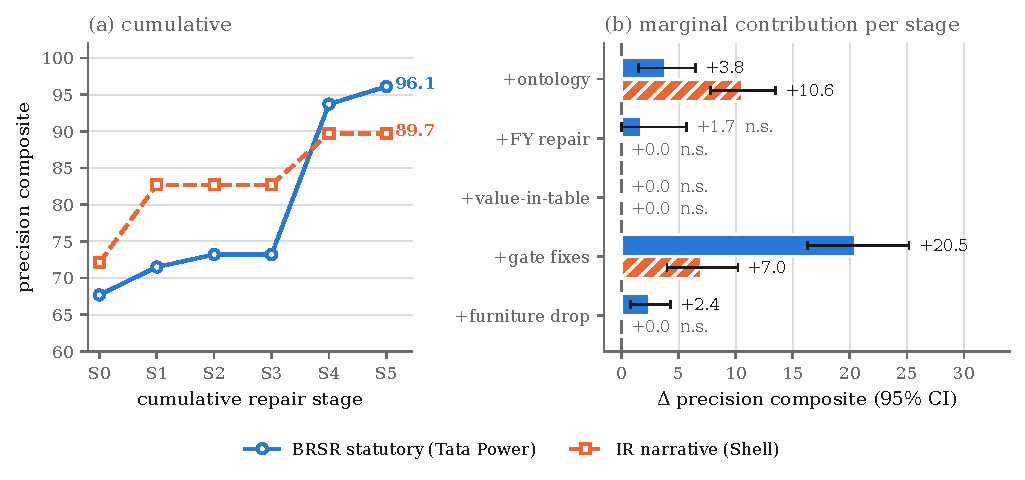
\includegraphics[width=\textwidth]{figures/fig1_ablation_by_regime.pdf}
\caption{Contribution of each deterministic repair stage by disclosure regime.
(a) cumulative precision composite; (b) marginal contribution per stage with
95\,\% confidence intervals from a paired bootstrap. The dominant stage differs by
regime and the two intervals do not overlap.}
\label{fig:ablation}
\end{figure*}

Three findings follow from Tables~\ref{tab:stages}--\ref{tab:deltas} and
Figure~\ref{fig:ablation}.

\paragraph{(i) The layer is worth $+24.6$ and $+7.0$ points at zero inference
cost.} We quote S1$\to$S5 rather than S0$\to$S5 deliberately. At S0 the aspect
node accuracy is $0\,\%$ \emph{by construction}---free text cannot exact-match a
controlled vocabulary---so the S0$\to$S5 totals ($+28.4$ and $+17.6$) partly
measure an artifact of comparing free text against a fixed taxonomy. S1, an LLM
plus a vocabulary mapping, is the minimum sane baseline, and the increment over
it is the defensible claim.

\paragraph{(ii) Only two of five components pay for themselves.} Fiscal-year
repair and source-value verification are indistinguishable from zero on both
documents. The method is more accurately described as \emph{taxonomy
normalisation plus rule-based repair} than as a five-stage pipeline. Fiscal-year
repair is arguably net-negative: Section~\ref{sec:recall} shows it also costs
$1.1$ percentage points of recall.

\paragraph{(iii) The dominant component is set by the disclosure regime.} On the
statutory filing the gate carries the result ($+20.5$; aspect node accuracy rises
from $18.9\,\%$ to $94.6\,\%$). On the narrative report it is taxonomy mapping
($+10.6$), and the furniture filter contributes nothing at all, because a
narrative report contains no statutory form furniture to remove. The intervals
for the two dominant levers do not overlap. This is the practical claim of the
paper: repair strategy must be matched to disclosure format, and a single
pipeline tuned on one regime will systematically under-serve the other.

\subsection{Cost}

The deterministic layer runs in $0.58$\,ms per claim---$218$\,ms for a 373-claim
report, single-threaded, no network, no API spend. Relative to an LLM
re-extraction pass this is effectively free, which is what makes finding (iii)
actionable: a deployment can afford to carry repair rules for every disclosure
regime it might encounter, and select among them per document.

\subsection{Recall, and what precision costs}
\label{sec:recall}

Against 482 table facts enumerated mechanically as described in
Section~\ref{sec:recall-method}, in the statutory filing the
shipped configuration achieves $54.4\,\%$ raw cell recall ($262/482$) and
$59.5\,\%$ distinct-fact recall; on the pages it processed at all, $57.8\,\%$.
Two pages produced no claims, accounting for 29 cells.

\begin{figure}[t]
\centering
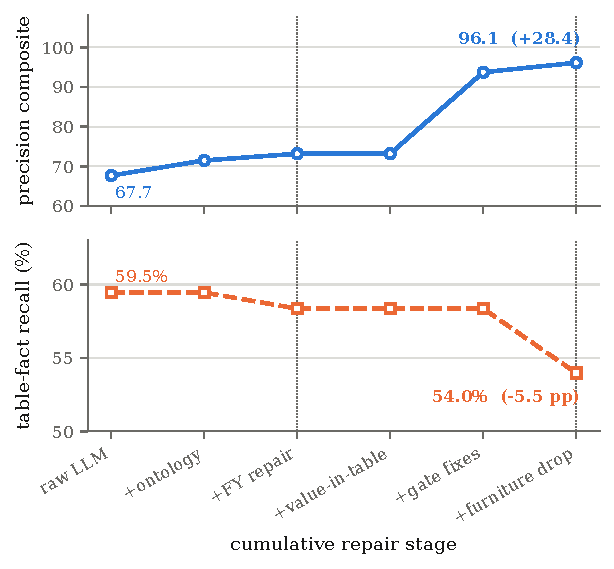
\includegraphics[width=\columnwidth]{figures/fig2_precision_recall_tradeoff.pdf}
\caption{Precision composite and table-fact recall across the same repair stages.
Panels share an x-axis rather than twinning y, since the two measures are not
commensurable. Precision rises 28.4 points while recall falls 5.5 percentage
points; dotted lines mark the two stages that cost recall.}
\label{fig:tradeoff}
\end{figure}

Figure~\ref{fig:tradeoff} makes the central practical caveat visible.
\textbf{Precision-oriented repair is a trade, not a free gain.} Across S0$\to$S5
the composite rises from $67.7$ to $96.1$ while distinct-fact recall
\emph{falls} from $59.5\,\%$ to $54.0\,\%$. The furniture filter removes 34
claims, and some of what it removes are genuine table facts. A precision-only
evaluation cannot observe this; a deployment tuned purely for precision will
silently drop real disclosures. We report recall for the statutory filing only:
the narrative fixture is text-dominant (13 table claims of 247) with partial page
coverage, so a table-recall figure computed from it would describe the fixture
rather than the pipeline.

\subsection{Baselines}

Two model-independent reference points bound the problem. A \textbf{rule-based
extractor with no LLM}, assigning aspects by taxonomy keyword matching, names
only $43.1\,\%$ of table rows; the remaining $57\,\%$ resolve to
\texttt{uncategorized}. That is the share of the tabular surface that genuinely
requires a model. \textbf{Grounding precision}---the share of emitted numeric
values that actually occur in the source page, a mechanical check comparable
across systems---is $87.4\,\%$ without the repair layer and $89.2\,\%$ with it.

\FILL{2x2 frontier-model comparison: does the repair delta survive a stronger
extractor? Run backend/scripts/run\_baselines.py --generate frontier and write
this subsection around the interaction term.}

%==============================================================================
\section{Limitations}
\label{sec:limitations}
%==============================================================================

Several of these bound what the results above can support, and we state them
rather than leaving them to be discovered.

\paragraph{Development sets, not held-out.} The taxonomy and repair rules were
tuned against both annotated sets. In one instance the change that raised the
narrative-report score also introduced taxonomy nodes named after concepts that
set had revealed, and revised two of its labels to match the new node names; a
later change revised four labels in the other set. Six of 100 labels have been
adjusted toward the system. \textbf{No untouched test set exists}, so no absolute
number here is evidence of generalisation. The paired ablation deltas are
unaffected---the stages are scored on identical claims---which is why we present
those as the primary result and the absolute scores as context. We have since
added a continuous-integration gate that fails the build when a gold label
changes without an explicit, documented version bump.

\paragraph{Single annotator.} All 100 labels were produced by one annotator, with
no second pass and no inter-annotator agreement statistic.

\paragraph{Precision-only composite.} The composite has no recall term and cannot
have one against sets sampled from extractor output. Measured table recall is
$59.5\,\%$ against the composite's $96.1$; the two describe the same pipeline.
Narrative-claim recall is unmeasured.

\paragraph{Parser-conditional recall.} Recall is relative to the units the parser
surfaced. Facts in unparsed figures or scanned tables lie outside the frame and
are not counted as misses.

\paragraph{Two documents.} The regime-divergence finding rests on one document
per regime. It supports a claim about these two disclosure formats, not about ESG
reporting in general.

\paragraph{Extraction is not reproducible end to end.} The extraction model is a
hosted endpoint at non-zero temperature. Frozen fixtures make every reported
number recomputable, but a fresh end-to-end run will not reproduce the corpus
exactly.

\paragraph{Scope.} The wider system also produces cross-report contradiction
flags, a greenwashing-signal taxonomy, a document-level integrity score and
satellite-imagery verification. \textbf{None of these is evaluated in this paper}
and we make no accuracy claim for any of them.

%==============================================================================
\section{Conclusion}
%==============================================================================

We measured the deterministic post-correction layer that sits between an LLM
extractor and a usable ESG claim store. It is worth $+24.6$ and $+7.0$ points of
a precision composite over an LLM-plus-vocabulary baseline, at $0.58$\,ms per
claim and no inference cost, and the gain is concentrated in two of five
components rather than spread across all of them.

The result we consider most useful is that the dominant component depends on the
disclosure regime, with non-overlapping confidence intervals: rule-based
correction carries a form-heavy statutory filing, taxonomy normalisation carries
a narrative report. Because the layer is essentially free to run, this argues for
carrying regime-specific repair rules and selecting among them per document
rather than tuning one pipeline and accepting degraded behaviour elsewhere. We
also showed that this repair is a trade---$5.5$ percentage points of table-fact
recall for $28.4$ points of precision composite---which a precision-only
evaluation cannot see.

Future work follows directly from Section~\ref{sec:limitations}. The most
important item is an annotation protocol anchored to source text units rather
than to extractor output, which would simultaneously yield a genuinely held-out
test set, make recall measurable for narrative claims, and decouple ground-truth
labels from the taxonomy so that ontology changes cannot propagate into the gold
standard. Beyond that: a second annotator with reported agreement, a wider corpus
spanning more disclosure regimes, and external validation of the downstream
integrity score against an independent criterion.

%==============================================================================
% \section*{Acknowledgements}   % <- RESTORE ONLY IN CAMERA-READY (deanonymising)
%==============================================================================

\bibliographystyle{elsarticle-num}
\bibliography{refs}

\end{document}
